\chapter{Motivation}
\label{ch:Motivation1}
 
Unternehmen treffen unzählige Entscheidungen jeden Tag. Wertschöpfende Entscheidungen tragen, wie ihr Name schon sagt, zur Wertschöpfung bei und beeinflussen somit unmittelbar den wirtschaftlichen Erfolg eines Unternehmens. Eine Bank beispielsweise muss einen Kreditnehmer auf dessen Fähigkeit, Raten zurückzahlen zu können, prüfen. Somit soll sichergestellt werden, dass die Bank den Betrag des Kredites sowie auch die ihr zustehenden Zinsen zurückbekommt. Dadurch steht und fällt der Erfolg einer Bank mit den Krediten, die sie vergibt \cite[vgl. S. 1]{AF04}. Prominentestes Beispiel hierfür ist die ehemalige US-amerikanische Investmentbank Lehmann Brothers, die im Zuge der Finanzkrise 2008 Insolvenz anmelden musste \cite[vgl. S. 3]{WN09}. Boomende Immobilien-Preise resultierten in höheren Sicherheiten von Privathaushalten, wodurch auch Kredite an Darlehnsnehmer mit geringer Bonität vergeben wurden (Subprime-Kredit) \cite[vgl. S. 82-83]{MB09}. Nach dem Platzen der Immobilienblase kam es zu Zahlungsausfällen und -störungen im US-amerikanischen Hypothekenmarkt \cite[vgl. S. 6 ff.]{RK10}, was erst in einem Finanzcrash und dann in einer Weltwirtschaftskrise resultierte \cite[vgl. S. 109]{LG09}.

Etwa im Juni 2009 waren die schlimmsten Auswirkungen der Finanzkrise überstanden, die amerikanische Wirtschaft begang wieder zu wachsen \cite[vgl. S. 21]{HR10} und Banken vergaben fleißig Kredite. Heutzutage werben Banken mit Kreditentscheidungen innerhalb von wenigen Sekunden. Das Ausfüllen eines Formulars ist ausreichend, um wenige Sekunden später eine Kreditentscheidung zu erhalten. Die Prüfung der Bonität geschieht automatisiert im Hintergrund durch eine zuvor definierte Entscheidungslogik. Die Entscheidungslogik wird von Fach-Experten erstellt, wobei die Fach-Experten im Wesentlichen zwei essentielle Dinge beachten:
 
\begin{enumerate*}
\item Verhinderung der Vergabe von Krediten an Personen, die diese 
nicht zurückzahlen können (''default rate'') 
\item Verhinderung der Nicht-Vergabe von Krediten an Personen, die eigentlich in der Lage 
sind, diese zurück zuzahlen, wodurch Einnahmen an Konkurrenten 
verloren gehen (''acceptance rate'') \end{enumerate*}

Banken sind somit angehalten eine gute Balance zwischen Sicherheit und Gewinn zu finden. Dazu muss die fachliche Entscheidungslogik drohende Zahlungsausfälle so genau wie möglich vorhersagen. Studien wie \cite[]{IM17} zeigen, dass sieben Prozent der vergebenen Kredite im Euroraum mehr als 90 Tage im Zahlungsverzug sind. Das entspricht einem Volumen von einer Billionen Euro. Bei einem Zahlungsverzug von über 90 Tagen wird generell davon ausgegangen, dass ein Kredit nicht mehr in voller Höhe zurückgezahlt wird und somit zu einem Verlust-Geschäft führt \cite[vgl. S. 8]{BF05}. Könnte man die Entscheidungslogiken bei den Banken dahingehend optimieren, ein Prozent weniger ''faule'' Kredite zu vergeben, könnten große Summen eingespart werden, die sonst im Zuge einer Banken-Rettung dem Steuerzahler auferlegt werden.        

\section{Problemstellung}
\label{sec:Problemstellung1}

Das Einsparen der genannten Summen wäre erstrebenswert, allerdings gibt es unzählige Gründe, die den Finanzcrash ab 2007 verschuldet haben. Als Hauptgrund wird in der Literatur die umfangreiche Vergabe von Subprime-Krediten genannt \cite[]{MB09, WN09}. Bei der Vergabe dieser Kredite wurde das Risiko nicht korrekt identifiziert \cite[vgl. S. 3]{WN09}, was zu unzähligen falschen fachlichen Entscheidungen führte. Daraus abgeleitet ergibt sich die Problemstellung dieser Arbeit, dass zu viele fachliche Entscheidungen falsch getroffen werden. Die Gründe hierfür werden nachfolgenden beschrieben und in Abbildung \ref{fig:Gruende} zusammengefasst.   

\begin{figure}[ht] 
\centering
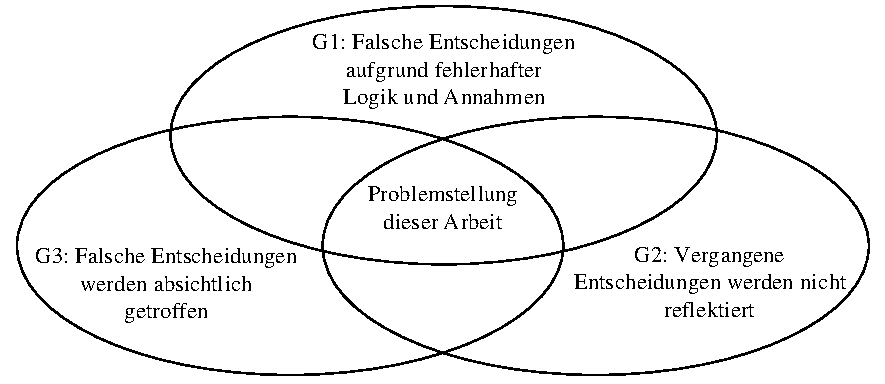
\includegraphics{images/gruende.pdf}
\caption{Gründe für falsch getroffene fachliche Entscheidungen.}
\label{fig:Gruende}
\end{figure}

Ein Grund für die vielen falschen Entscheidungen, sind fehlerhafte Entscheidungslogiken und falsche Annahmen (Grund G1 - siehe Abbildung \ref{fig:Gruende}). Bei der Vergabe der Kredite wurden die Entscheidungen verfälscht, da die Entscheidungslogiken mit Eingabe-Daten befüllt wurden, die nicht der Realität entsprachen. Durch die unrealistisch hohen Immobilien-Preise, waren die Kredite mit Immobilien gesichert, die real weitaus weniger wert waren \cite[]{HR11}. Die Kredite wurden dementsprechend auf Basis von nicht vorhandenen Sicherheiten berechnet.

Ein weiterer Grund ist, dass vergangene Entscheidungen nicht mehr reflektiert wurden. (Grund G2 - siehe Abbildung \ref{fig:Gruende}). Die Kredite wurden gebündelt unter den Banken weiterverkauft \cite[vgl. S. 2]{WN09}, ein Verlust-Risiko bestand somit nur für die kurze Zeit, in der ein Kredit-Bündel noch nicht weiterverkauft wurde. Saunders et al. sagen ''The underwriters [...] had little incentive to screen and monitor the activities of borrowers for whom they originated loans'' \cite[]{SA10}. Nach der ursprünglichen Vergabe des Kredites, wurden also keine weitere Aktivitäten unternommen, um die damaligen Kredit-Entscheidungen weiterhin zu prüfen oder zu überwachen. Ein Kontrollverlust der Situation war nur eine Frage der Zeit.            

Im Falle der Finanzkrise waren allerdings nicht nur fehlerhafte Entscheidungslogik, falsche Annahmen und mangelnde Reflektion schuld am Zusammenbrauch der Finanzmärkte. Absichtlich falsch getroffene Entscheidungen sind ebenso als Ursache der vielen falsch getroffenen Entscheidungen anzuführen (Grund G3 - siehe Abbildung \ref{fig:Gruende}). In einer Pressemitteilung des Vorstandes der US-Notenbank, wurden Bonus-Zahlungen an Bank-Mitarbeiter als weiterer Grund der Finanzkrise aufgezählt: ''Flaws in incentive compensation practices were one of many factors contributing to the financial crisis. Inappropriate bonus or other compensation practices can incent senior executives or lower level employees, such as traders or mortgage officers, to take imprudent risks that significantly and adversely affect the firm'' \cite[]{BG09}. Mitarbeiter übertraten bewusst Risiken, nutzten mangelnde Regulationen zu ihrem Vorteil und ließen keine Möglichkeit aus ihren Gewinn auf Kosten von Stabilität und Sicherheit zu maximieren. 

Zusammenfassend soll Abbildung \ref{fig:Gruende} nochmals die Gründe aufzeigen die verantwortlich sind, dass zu viele falsche fachliche Entscheidungen getroffen werden.

\section{Zielsetzung}
\label{sec:Zielsetzung1}

Das übergeordnete Ziel ist die in \ref{sec:Problemstellung1} genannte Problemstellung, dass zu viele falsche fachliche Entscheidungen getroffen werden, zu verbessern, indem man die Anzahl falscher fachlichen Entscheidungen reduziert. Diese Arbeit soll hierzu ein Machine Learning (ML) Verfahren evaluieren, analysieren und implementieren, um fachliche Entscheidungen zu verbessern. Aus dieser Zielsetzung können die folgenden Teilziele abgeleitet werden. 

Das \textit{erste Teilziel} ist das Erstellen und die kontinuierliche Optimierung von Modellen, anhand von vergangen fachlichen Entscheidungen und deren Korrektheit. Dazu soll im ersten Schritt ein ML-Verfahren implementiert werden, das Modelle aus den Daten vergangener Entscheidungen generiert. Die Datensätze dieser Entscheidungen werden um ein weiteres Attribut ergänzt, die Performance. Die Performance beschreibt den Fall, der sich in der realen Welt als der richtige erwiesen hat. Bei der Kredit-Entscheidungslogik beispielsweise, wäre die Performance ob ein Kunde seinen Kredit zurückgezahlt hat oder nicht. Das ML-Verfahren, soll die Kombination von Input-Daten und Performance auf Gesetzmäßigkeiten prüfen und diese anschließend als Modell zur Verfügung stellen. Ein Modell beschreibt den Output eines ML-Verfahrens und bietet zwei fundamentale Mechanismen. Erstens soll das Modell in der Lage sein, weiter optimiert werden zu können (''lernen''), zweitens soll für einen gegebenen Input-Datensatz ein dazugehörender Output vorhergesagt werden (''evaluieren''). 

Das \textit{zweite Teilziel} besteht darin Modelle heranzuziehen, um Entscheidungslogiken so zu verbessern, dass zukünftige fachliche Entscheidungen korrekter getroffen werden. Das erlernte Modell wird  dazu verwendet, mehrere Datensätze zu evaluieren und den Ausgang deren Entscheidungen vorherzusagen. Die daraus resultierenden Ergebnisse sollen dann in den Entscheidungsfindungsprozess mit einfließen und somit zu mehr richtig getroffenen Entscheidungen verhelfen. 

Auf Basis dieser Teilziele ergeben sich eine Reihe von Forschungsfragen: 

\begin{itemize*}
\item \textbf{Forschungsfrage 1:} Können ML-Verfahren verwendet werden, um fachliche Entscheidungen zu verbessern? 

- Was gibt es für einsetzbare ML-Verfahren?

- Welche ML Verfahren eignen sich am besten?

\item \textbf{Forschungsfrage 2:} Wie können einsetzbare ML-Verfahren anhand eines fachlichen Anwendungsfall angewendet werden? 

- Welche Anwendungsfälle eignen sich hierzu?

- Was für Ergebnisse liefern diese? 

- Wie können die Ergebnisse interpretiert werden?

\item \textbf{Forschungsfrage 3:} Wie kann die Funktionsweise des ML-Verfahrens in ein Modell überführt werden, ohne dass dabei Performance-Daten offen gelegt oder zur Verfügung gestellt werden müssen?

\item \textbf{Forschungsfrage 4:} Wie kann sichergestellt werden, dass die fachliche Entscheidung verbessert werden können?
\end{itemize*}


Die vier Forschungsfragen werden in Tabelle /ref{tab:chapters} 1.2 zu einem oder mehreren Kapiteln dieser Thesis zu geordnet. 

\begin{table}[htb]
\centering
\small
\begin{tabular}{lccccccc}
\toprule
\# & Kap. 1 & Kap. 2 & Kap. 3 & Kap. 4 & Kap. 5 & Kap. 6 & Kap. 7\\
\toprule
Forschungsfrage 1 &  & $\times$ & & &$\times$& &\\\midrule
Forschungsfrage 2 &  &$\times$& $\times$ & $\times$ & & &\\\midrule
Forschungsfrage 3 &  & &  $\times$ & $\times$& & &\\\midrule
Forschungsfrage 4 &  &  $\times$& $\times$ &  $\times$&$\times$  & &\\\bottomrule
\end{tabular}
\caption{Forschungsfragen entlang der Kapitel.}
\label{tab:chapters}
\end{table}

\section{Abgrenzung}
\label{sec:Abgrenzung1}

Einhergehend mit den zu beantwortenden Forschungsfragen findet auch folgende Abgrenzung statt: Es ist kein Ziel dieser Arbeit, einen eigenen ML-Algorithmus zu entwickeln. Die Entwicklung eines eigenen Algorithmus ist nicht notwendig, da in der Literatur und Praxis schon vielversprechende Algorithmen entwickelt worden sind. Vielmehr sollen bereits bestehende Algorithmen und Lösungen, die sich in der Praxis als erfolgreich bewiesen haben, intelligent verknüpft werden, um fachliche Entscheidungen zu verbessern.  Ziel dieser Arbeit ist ausschließlich das Verbessern von automatisierbaren Entscheidungen. Entscheidungen können operativer und strategischer Natur sein, wobei sich nur operative Entscheidungen zur Automatisierung eignen. 
    
\section{Aufbau der Arbeit}
\label{sec:Aufbau_der_Arbeit1}

Die vorliegende Bachelorarbeit besteht aus sieben Kapiteln, die sich nochmals in drei Teile (Teil I - Teil III) aufgliedern (siehe Abbildung \ref{fig:Aufbau}).

\begin{figure}[ht]
\centering
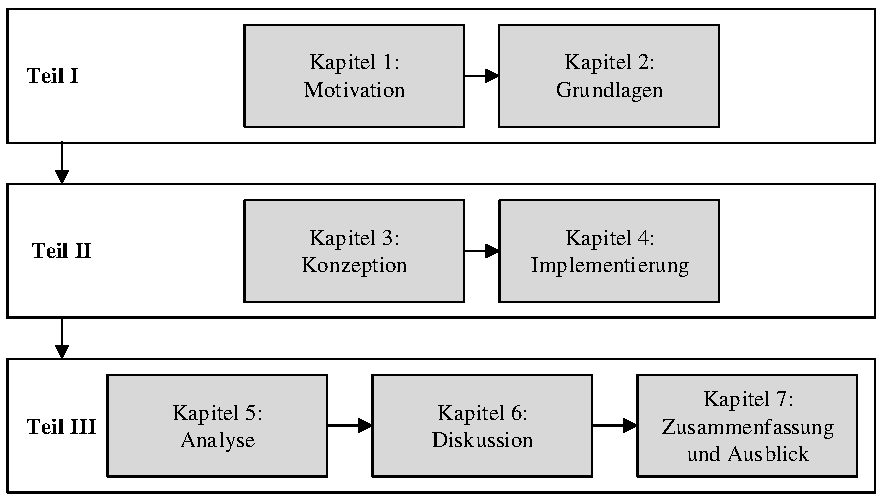
\includegraphics{images/Aufbau.pdf}
\caption{Aufbau der Arbeit.}
\label{fig:Aufbau}
\end{figure}

\textbf{Teil 1} umfasst neben diesem einleitenden Kapitel die theoretischen Grundlagen, die für das weitere Verständnis benötigt werden. Kapitel \ref{sec:Decision_Management2} erläutert wie Entscheidungen abgebildet werden können, anschließend werden die Grundlagen von ML vermittelt (Kapitel \ref{sec:Machine_Learning2}), um im Anschluss verwendbare Technologien für Decison Management und ML zu identifizieren (Kapitel \ref{sec:Technologien2}).  

\textbf{Teil 2} befasst sich mit der Konzeption des Prototypen (Kapitel 3), sowie dessen Implementierung (Kapitel 4) und stellt damit den Hauptteil dieser Arbeit dar. Hierzu sollen zuerst Anwendungsfälle genannt werden (Kapitel 3.1), wovon anschließend Anforderungen abgeleitet und spezifiziert werden (Kapitel 3.2). Mit dem Abschluss der Konzeption, wird die Implementierung des Prototypen beschrieben. Hierzu wird zunächst die Implementierung des Datenschemas dargelegt (Kapitel 4.1), bevor die Implementierung der zu verbessernden Entscheidungslogik (Kapitel 4.2) erläutert wird. Aufbauend auf der Entwicklung des Datenschemas und der Entscheidungslogik, kann das ML-Verfahren implementiert (Kapitel 4.3) und optimiert werden (Kapitel 4.4).        

\textbf{Teil 3} bildet den Schlussteil der Arbeit und umfasst die Analyse (Kapitel 5), die Diskussion (Kapitel 6) und die Zusammenfassung inklusive eines Ausblicks (Kapitel 7).

